\section{Theory}
\label{sec:theory}
We model action editing with a latent video-generating process, establish
when paired-view learning identifies action anchors, and explain their role
in demonstration-guided editing.

\subsection{Problem formulation}
\label{subsec:dgp-overview}

For a video $V=(\mathbf x_1,\ldots,\mathbf x_T)$, let $\mathbf z^{\mathrm c}$
denote persistent content and $\mathbf z^{\mathrm a}_t$ its action state.
For a controlled description with physical context fixed, the generating process is
\begin{equation}
 \begin{aligned}
  \mathbf z^{\mathrm c}&\sim p_{\mathrm c},\qquad (u,\mathbf z^{\mathrm a}_0,\boldsymbol\epsilon_{1:T})\sim p_{\mathrm{dyn}},\\
  \mathbf z^{\mathrm a}_t&=f(\mathbf z^{\mathrm a}_{t-1},u,\boldsymbol\epsilon_t),\qquad
  V=g_{\mathrm{ctrl}}(\mathbf z^{\mathrm c},\mathbf z^{\mathrm a}_{0:T}).
 \end{aligned}
 \label{eq:dgp-controlled}
\end{equation}
Here, $u$ specifies the action regime (e.g., raising or lowering an arm),
and $\boldsymbol\epsilon_t$ captures stochastic variation in the state
transition $f$. The observation map $g_{\mathrm{ctrl}}$ maps content and
the resulting action trajectory to a video. $p_{\mathrm c}$ is the content
distribution, while $p_{\mathrm{dyn}}$ is the joint distribution of $u$,
the initial state $\mathbf z^{\mathrm a}_0$, and $\boldsymbol\epsilon_{1:T}$.
The action block is $\mathbf z^{\mathrm a}:=\mathbf z^{\mathrm a}_{0:T}$.
Content is independent of the action-generating variables
(Appendix~\ref{sec:controlled-transfer}). For source
$V_{\mathrm s}=g_{\mathrm{ctrl}}(\mathbf z^{\mathrm c}_{\mathrm s},\mathbf z^{\mathrm a}_{\mathrm s})$ and demonstration
$V_{\mathrm r}=g_{\mathrm{ctrl}}(\mathbf z^{\mathrm c}_{\mathrm r},\mathbf z^{\mathrm a\star})$, the desired edit is
\begin{equation}
 V^\star=g_{\mathrm{ctrl}}(\mathbf z^{\mathrm c}_{\mathrm s},\mathbf z^{\mathrm a\star}).
 \label{eq:dgp-counterfactual}
\end{equation}
Action-preserving pairs vary appearance at a fixed trajectory
(Figure~\ref{fig:controlled-dgp}). We use this relation to study when
an action representation can be recovered independently of appearance.

\begin{figure}[!htbp]
 \centering
 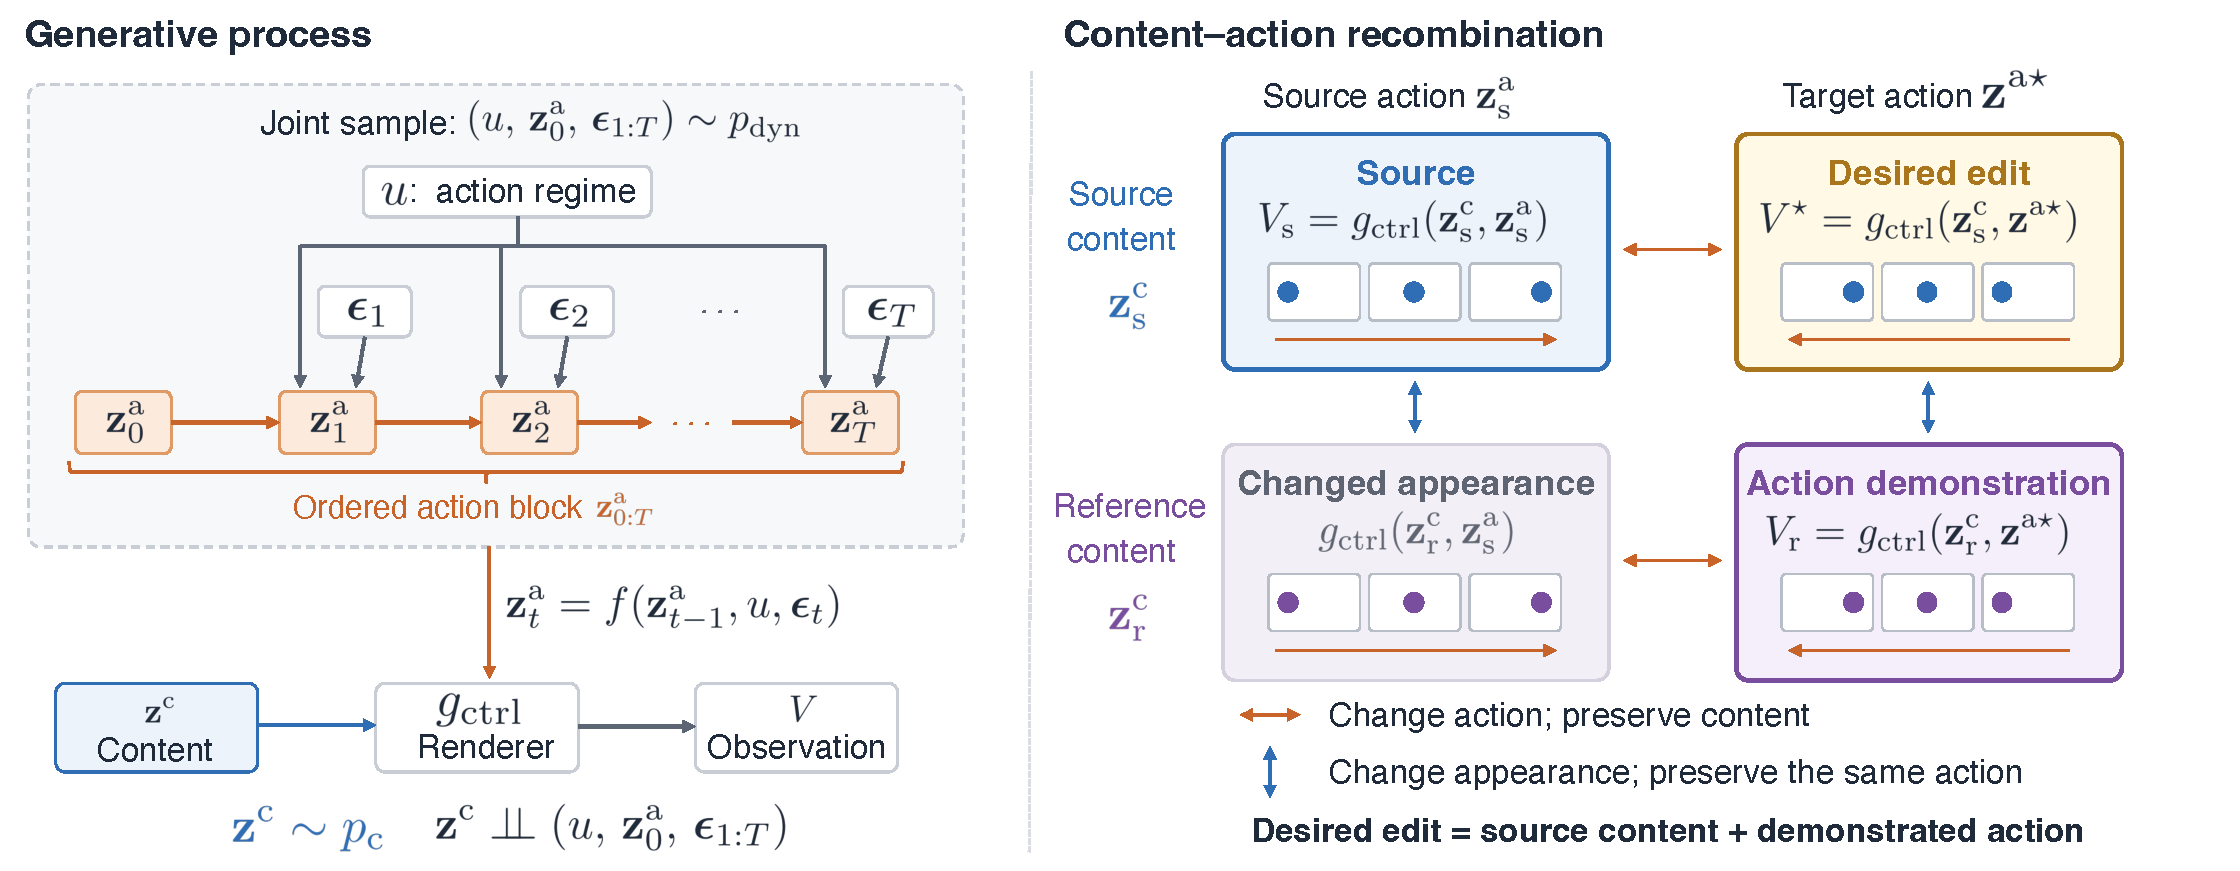
\includegraphics[width=\linewidth]{data_generating_process.pdf}
 \caption{Controlled video generation and content--action recombination within a fixed physical context.
 Content $\mathbf z^{\mathrm c}$ and action $\mathbf z^{\mathrm a}_{0:T}$ jointly determine the video
 through the renderer $g_{\mathrm{ctrl}}$ (left).
 Rows share content and columns share action; the desired edit combines source content
 $\mathbf z^{\mathrm c}_{\mathrm s}$ with demonstrated action $\mathbf z^{\mathrm a\star}$ (right).}
 \label{fig:controlled-dgp}
\end{figure}
\subsection{Learning identifiable action anchors}
\label{subsec:anchor-learning}
\label{subsec:anchor-identification}

A demonstration supplies temporal behavior together with its visual content.
The learning problem is to retain the former across changes in the latter.
Let $\mathbf w$ collect the initial state, regime, and innovations in
Eq.~\ref{eq:dgp-controlled}, and let $\mathcal F_T(\mathbf w)=\mathbf z^{\mathrm a}_{0:T}$
be its unrolled trajectory. An action-preserving pair holds $\mathbf w$ fixed:
\begin{equation}
 V=g_{\mathrm{ctrl}}(\mathbf z^{\mathrm c},\mathcal F_T(\mathbf w)),\qquad
 V^+=g_{\mathrm{ctrl}}(\mathbf z^{\mathrm c+},\mathcal F_T(\mathbf w)).
 \label{eq:controlled-anchor-views}
\end{equation}
The entire realized trajectory is shared, including timing and interactions;
an action label alone does not specify this relation. These are
representation-learning pairs; the source and target-action demonstration
may depict different actions.

\begin{definition}[Blockwise identification]
\label{def:anchor-identification}
An encoder $E_{\mathrm a}:\mathcal V\to\R^{d_{\mathrm a}}$ identifies the action block if
$E_{\mathrm a}(V)=h_{\mathrm a}(\mathbf z^{\mathrm a})$ almost surely,
where $h_{\mathrm a}$ is injective on a full-measure subset of the action support.
Coordinates may mix within the block.
\end{definition}

\Needspace{13\baselineskip}
\begin{condition}[Nonlinear action identification]
\label{cond:anchor-identification}
\leavevmode

\par\noindent\textup{(i)} \textbf{Regularity.}
The supports $\mathcal W$ and $\mathcal Z^{\mathrm c}$ are compact, and
$f$ and $g_{\mathrm{ctrl}}$ are continuous. Write
$\mathcal A_T=\mathcal F_T(\mathcal W)$ for the supported trajectory family.

\par\noindent\textup{(ii)} \textbf{Appearance variation.}
The two content variables in Eq.~\ref{eq:controlled-anchor-views} are
independent draws from $p_{\mathrm c}$, independently of $\mathbf w$,
and $p_{\mathrm c}$ has full support on $\mathcal Z^{\mathrm c}$.

\par\noindent\textup{(iii)} \textbf{Temporal observability.}
Two distinct trajectories in $\mathcal A_T$ cannot generate the same
complete video under any supported content choices.
\end{condition}
Part (iii) concerns the ordered video, not each frame separately.
An injective video-generating map suffices, but recovering content is
unnecessary. The observation map may mix action and appearance nonlinearly;
no additive feature decomposition is imposed.

\paragraph{Population learning problem.}
Agreement alone permits collapse, while predicting an ordinary feature
mean can erase differences between actions. We therefore analyze prediction
of the action-conditional video distribution. Let $k$ be a bounded,
continuous characteristic kernel on ordered videos, with feature map
$\varphi(V)=k(V,\cdot)$ in its reproducing kernel Hilbert space $\mathcal H_k$.
``Characteristic'' means that the mean embedding uniquely determines a
probability distribution; a Gaussian kernel on vectorized videos is one
choice~\citep{sriperumbudur2010hilbert}. Consider
\begin{equation}
 \begin{aligned}
 \mathcal J(E_{\mathrm a},P)
 ={}&\lambda\,\underbrace{\E\|E_{\mathrm a}(V)-E_{\mathrm a}(V^+)\|^2}_{\mathcal L_{\mathrm{inv}}}\\
 &+\underbrace{\E\|P(E_{\mathrm a}(V))-\varphi(V^+)\|_{\mathcal H_k}^2}_{\mathcal L_{\mathrm{pred}}},
 \qquad\lambda>0 .
 \end{aligned}
 \label{eq:anchor-objective}
\end{equation}
We optimize over all continuous encoders and measurable predictors
with finite risk. The code dimension must admit continuous
injective coordinates of $\mathcal A_T$; the full trajectory always
provides such coordinates. This criterion uses observed view pairs
without action-coordinate labels.

\begin{theorem}[Blockwise identification by paired-view learning]
\label{thm:anchor-identification}
Under Eq.~\ref{eq:controlled-anchor-views} and
Condition~\ref{cond:anchor-identification}, the population class above
attains the minimum of Eq.~\ref{eq:anchor-objective}.
Every global minimizer satisfies
\begin{equation}
 E_{\mathrm a}(V)=h_{\mathrm a}(\mathbf z^{\mathrm a}),\qquad
 P(h_{\mathrm a}(\mathbf z^{\mathrm a}))=\mu_k(\mathbf z^{\mathrm a})
 \quad\text{almost surely},
 \label{eq:anchor-identification}
\end{equation}
where $\mu_k(\mathbf a)=\E[\varphi(V)\mid\mathbf z^{\mathrm a}=\mathbf a]$
and $h_{\mathrm a}$ is injective on a full-measure action subset.
\end{theorem}

\paragraph{Proof sketch.}
Temporal observability and compactness give a continuous action readout
from the whole video. Distinct actions induce distributions supported on
disjoint sets of videos, so their characteristic embeddings differ.
These facts construct an invariant encoder and predictor attaining the
irreducible prediction variance. Conditional independence decomposes the
objective into this variance and two nonnegative errors. Every global
optimum therefore eliminates appearance variation while retaining distinct
action distributions (Appendix~\ref{subsec:nonlinear-anchor-proof}).

\subsection{Temporal information and action transfer}
\label{subsec:anchor-realization}

Consider position--velocity dynamics with constant acceleration $u$ and
nonlinear frame observations
\[
 p_t=p_0+t v_0+\tfrac12t^2u,\qquad \mathbf x_t=\rho(c,p_t),
\]
where $\rho$ is any continuous invertible map with continuous inverse
on the supported inputs. Three distinct observation times determine
$(p_0,v_0,u)$ and the full trajectory, whereas two times leave an ambiguity.
Thus single-frame recovery of the action block is unnecessary, even when
appearance and position interact nonlinearly
(Appendix~\ref{subsec:nonlinear-temporal-example}).

For additive features, the prediction target can be simplified. On the
supported content--trajectory pairs, let
\[
 \Phi(V)=q_{1:T}(\mathbf z^{\mathrm a})+\mathbf D r(\mathbf z^{\mathrm c}),
 \qquad
 \mathcal N_T=\operatorname{im}\Cov(\mathbf D r(\mathbf z^{\mathrm c})),
\]
where $\mathbf D$ is fixed, $q_{1:T}$ stacks the framewise action responses
$q_t$, and $\mathcal N_T$ is the subspace of appearance variation.

\begin{corollary}[Identification from additive features]
\label{cor:additive-anchor-learning}
Assume Condition~\ref{cond:anchor-identification}(i)--(ii), continuous
$\Phi,q_t$, and finite covariance of $r(\mathbf z^{\mathrm c})$.
Suppose $q_{1:T}(\mathbf a)-q_{1:T}(\mathbf a')\notin\mathcal N_T$
for any distinct $\mathbf a,\mathbf a'\in\mathcal A_T$.
Over the population model class above, with
$d_{\mathrm a}\geq\operatorname{rank}\Cov(\Phi(V))-\dim\mathcal N_T$,
every global minimizer of Eq.~\ref{eq:anchor-objective} with
$\varphi(V^+)$ replaced by $\Phi(V^+)$ and squared Euclidean prediction
error identifies the action block.
\end{corollary}

Averaging over appearance leaves an injective function of the action
trajectory, allowing ordinary feature prediction to identify the action
block (proof in Appendix~\ref{subsec:anchor-proof-identification}).
